Sections \S3--\S5 all share one property: they modify or fine-tune a pre-trained network's weights. Visual Prompt Tuning \citep{jia2022vpt} does something different. It freezes the entire backbone and inserts a small set of learnable \emph{prompt tokens} into the input space of a Vision Transformer, training only those prompts plus the classifier head. We test both variants from the original paper.

\subsection{VPT-Shallow}
VPT-Shallow inserts prompts only at the first Transformer layer. Given an image embedded into patch tokens $E_0 = [e_0^1, \dots, e_0^m]$ and a classification token $x_0$, VPT-Shallow prepends $p$ learnable prompts $P = [\mathbf{p}^1, \dots, \mathbf{p}^p]$:
\[
  [x_1, Z_1, E_1] = L_1([x_0, P, E_0]),
\]
where $L_1$ is the first frozen Transformer layer and $Z_1$ are the processed prompt outputs (discarded). The remaining layers receive $[x_i, Z_i, E_i]$ unchanged. Only $P$ and the classifier head are trained.

We use ViT-B/16 pre-trained on ImageNet-1k as the backbone and $p = 10$ prompts. Trainable parameter count: 86,118.

\subsection{VPT-Deep}
VPT-Deep inserts fresh prompts at \emph{every} Transformer layer:
\[
  [x_i, \_, E_i] = L_i([x_{i-1}, P_{i-1}, E_{i-1}]),
\]
where $P_{i-1}$ is a layer-specific learnable prompt matrix. The prompts from the previous layer are discarded at each step, so only $P_0, \dots, P_{N-1}$ and the classifier head are trained. With $p = 10$ and 12 Transformer layers, the model has 170,598 trainable parameters, which is 0.2\% of the ViT-B/16 backbone.

\subsection{Results and Analysis}
\begin{table}[H]
\centering
\small
\begin{tabular}{lcccc}
\toprule
Method & Test Acc (\%) & MPC Acc (\%) & Top-5 (\%) & Trainable params \\
\midrule
VPT-Deep    & \textbf{91.64} & \textbf{92.83} & \textbf{97.93} & 170,598 \\
VPT-Shallow & 84.13 & 85.70 & 95.43 & 86,118 \\
Frozen ResNet18 (best CNN) & 88.52 & 90.82 & --- & 10,545,766 \\
\bottomrule
\end{tabular}
\caption{Visual Prompt Tuning versus the best CNN we tuned.}
\label{tab:vpt-results}
\end{table}

VPT-Deep beats every CNN configuration we trained, including the frozen-layer ResNet18 that won \S4. It does so with 62$\times$ fewer trainable parameters than the frozen ResNet18 and 139$\times$ fewer than full ResNet18 fine-tuning. Top-5 accuracy of 97.93\% means the correct class is among the top five predictions for all but 2\% of test images.

VPT-Shallow (85.70\% MPC) is competitive with the unmodified ResNet18 baseline (86.11\%) but falls short of the best CNN. This matches the pattern reported in the original VPT paper: shallow prompts alone do not provide enough capacity for fine-grained recognition, and inserting prompts at every layer is worth the extra 85K parameters.

\textbf{Prompt length ablation.} Figure~\ref{fig:prompt-length} varies the number of prompts per layer for VPT-Deep. Accuracy increases monotonically from $p=1$ (91.08\% val) to $p=50$ (94.51\% val). Our default $p=10$ gives 93.63\%. Longer prompts continue to help, but with diminishing returns and more parameters.

\begin{figure}[H]
\centering
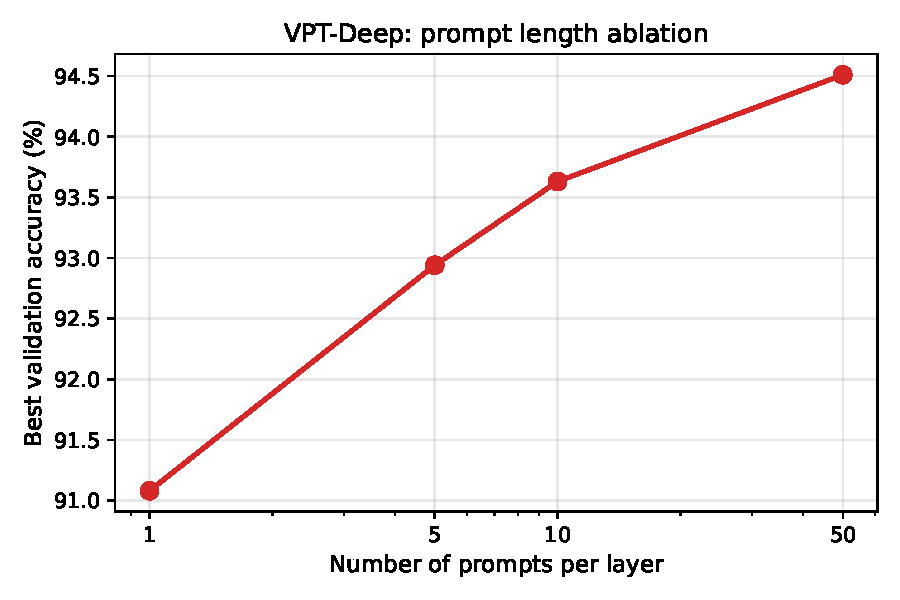
\includegraphics[width=0.65\textwidth]{figures/prompt-length.pdf}
\caption{VPT-Deep accuracy vs.\ number of prompts per layer.}
\label{fig:prompt-length}
\end{figure}
